\documentclass[12pt, oneside]{article}
\usepackage[letterpaper, margin=1in, headsep=0.5in, left=0.3in, right=2.5in]{geometry}
\usepackage[english]{babel}
\usepackage[utf8]{inputenc}
\usepackage{amsmath}
\usepackage{amsfonts}
\usepackage{amssymb}
\usepackage{tikz}
\usepackage{yhmath}
\usetikzlibrary{quotes, angles}
\usepackage{graphicx}
\usepackage{enumitem}
\usepackage{multicol}

\newif\ifmeta
\metatrue %print standards and topics tags

\title{Regents Geometry}
\author{Chris Huson}
\date{April 2022}

\usepackage{fancyhdr}
\pagestyle{fancy}
\fancyhf{}
\renewcommand{\headrulewidth}{0pt} % disable the underline of the header
\raggedbottom

%\fancyhead[LE]{\thepage}
\fancyhead[RO]{Name:}
\fancyhead[LO]{BECA / Dr. Huson / Geometry Regents Mixed Review}
\cfoot{\thepage}

\begin{document}
\subsubsection*{11.10 Circle equations and secants}
\begin{enumerate}[itemsep=2cm]
\item What is an equation of the image of the line $\displaystyle y=-x-8$ after a dilation with a scale factor of $\displaystyle \frac{7}{4}$ centered at the origin?

\item The equation of a cirle is $x^2+y^2+8x-12y=12$. What are the center and radius of the circle? \vspace{1cm}

\item Which equation represents a line that is perpendicular to the line represented by\\[0.25cm] $\displaystyle y=-\frac{1}{3}x+7$?
  \begin{multicols}{2}
    \begin{enumerate}
      \item $3x+y=10$
      \item $3x-y=10$ 
      \item $\displaystyle y=-\frac{1}{3}x+2$
      \item $\displaystyle y=\frac{1}{3}x+4$
    \end{enumerate}
  \end{multicols}

\item In the diagram below of right $\triangle ABC$ , $\sin A =\cos B$, $m\angle A = 6x$, and $m\angle B = 3x$. Find $x$.
\begin{center}
  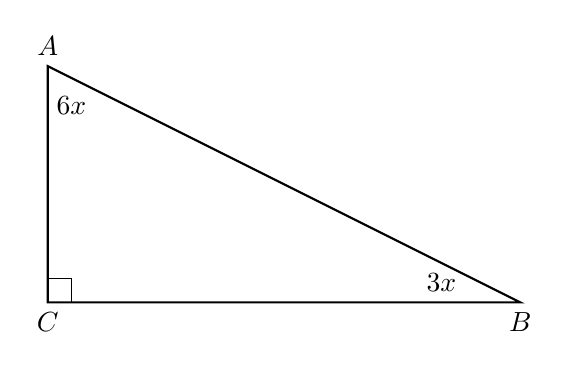
\begin{tikzpicture}[scale=1]
  \draw [thick]
    (-1,-1)node[below]{$B$}--
    (-7,2)node[above]{$A$}--
    (-7,-1)node[below]{$C$}--cycle;
    \draw (-7,-1)++(0.3,0)--++(0,0.3)--+(-0.3,0);
    \node at (-6.7,1.5){$6x$};
    \node at (-2,-0.75){$3x$};
\end{tikzpicture}
\end{center}

\newpage
\item The secants $\overline{ABC}$ and $\overline{ADE}$ intersect the circle $O$, as shown in the diagram. \\Given $m \wideparen{BD}=36^\circ$ and $m \wideparen{CE}=138^\circ$.
  \begin{enumerate}
    \item Find the $m\angle CDE$, $m\angle CBE$.
    \item Find the $m\angle C$, $m\angle E$.
    \item Find the $m\angle A$.
    \item Two similar triangles are shown. Write a similarity statement, listing the triangles' vertices in corresponding order.
  \end{enumerate}
  \begin{center}
  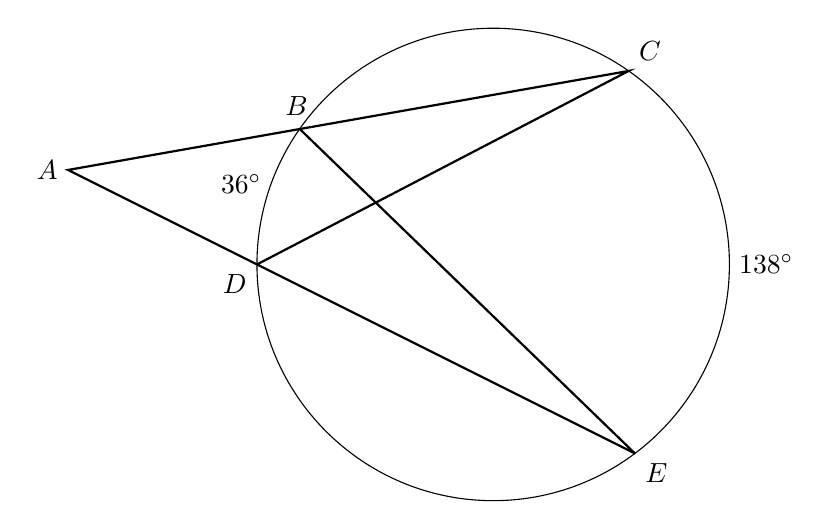
\begin{tikzpicture}[scale=.6]
    \draw (0,0) circle[radius=5];
    \draw [thick]
    (3,-4) node[below right] {$E$}--
    (-5,0) node[below left] {$D$}--
    (-9,2) node[left] {$A$}--
    (55:5) node[above right] {$C$}--
    (-5,0);
    \draw [thick] (3,-4)--(145:5);
    \draw (138:5) node[left] {$B$};
    \draw (0:5) node[right] {$138^\circ$};
    \draw (160:5) node[left] {$36^\circ$};
  \end{tikzpicture}
  \end{center}

\item In the diagram below of $\triangle RST$, $L$ is a point on $\overline{RS}$, and $M$ is a point on $\overline{RT}$, such that $\overline{LM} \parallel \overline{ST}$.
\begin{center}
\begin{tikzpicture}[scale=0.7]
  \draw [thick]
  (0,0) node[below] {$R$}--
  (45:10) node[above right] {$T$}--
  (4,0) node[below] {$S$}--cycle;
  \draw [thick]
  (45:2.5) node[above] {$M$}--
  (1,0) node[below] {$L$};
\end{tikzpicture}
\end{center}
If $RM=4$, $MT=12$, and $ST=15$, what is the length of $\overline{LM}$?

\end{enumerate}
\end{document}
  